%%%%%%%%%%%%%%%%%%%%%%%%%%%%%%%%%%%%%%%%%%%%%%%%%%%%%%%%%%%%%%%%%%%%%%%%%%%%%%%%%%
\begin{frame}[fragile]\frametitle{}
\begin{center}
{\Large Yoga for Health Promotion }
\end{center}
\end{frame}


%%%%%%%%%%%%%%%%%%%%%%%%%%%%%%%%%%%%%%%%%%%%%%%%%%%%%%%%%%%
\begin{frame}[fragile]\frametitle{Syllabus}

\begin{itemize}
\item 3.1  Brief introduction to human body. 
\item 3.2  Meaning and Means of health promotion and role of Yoga  in health promotion. 
\item 3.3  Yogic positive attitudes ( Maîtri, Karuna, Mudita, Upeksha). 
\item 3.4  Concept of bhavas (Dharma, Jnana, Vairagya, Aishvarya) and their relevance in well being. 
\item 3.5  Dincharya and Ritucharya with respect to Yogic life style. 
\item 3.6  Holistic approach of Yoga towards health and diseases. 
\item 3.7  Introduction to First aid and Cardio Pulmonary Resuscitation (CPR). 
\item 3.8  Yogic management of stress and its consequences. 
\item 3.9  Yoga in prevention of metabolic and respiratory disorders. 
\item 3.10  Yoga for personality development. 
\end{itemize}
	  
\end{frame}

%%%%%%%%%%%%%%%%%%%%%%%%%%%%%%%%%%%%%%%%%%%%%%%%%%%%%%%%%%%%%%%%%%%%%%%%%%%%%%%%%%
\begin{frame}[fragile]\frametitle{}
\begin{center}
{\Large Anatomy}
\end{center}
\end{frame}

%%%%%%%%%%%%%%%%%%%%%%%%%%%%%%%%%%%%%%%%%%%%%%%%%%%%%%%%%%%
\begin{frame}[fragile]\frametitle{Components of the Skeletal System}
\begin{columns}
    \begin{column}[T]{0.5\linewidth}
      \begin{itemize}
		\item Bones: 206 in adults, living organs, rich blood supply
		\item Cartilage: Elastic tissue, cushions joints
		\item Ligaments: Bind bones at joints
		\item Tendons: Connect muscles to bones
		\item Joints: Points of bone contact
	  \end{itemize}
    \end{column}
    \begin{column}[T]{0.5\linewidth}
		\begin{center}
		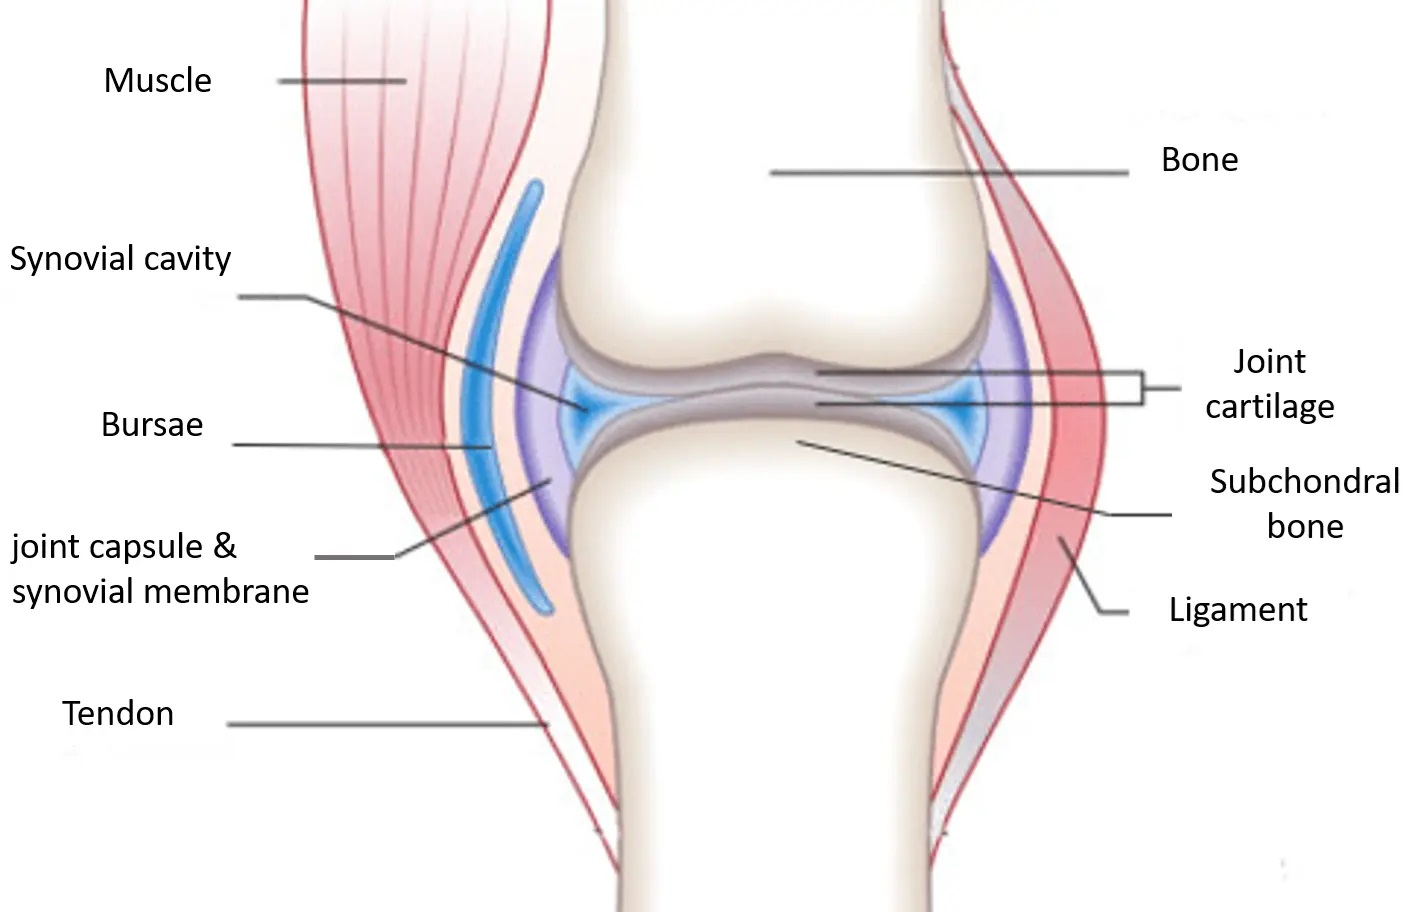
\includegraphics[width=\linewidth,keepaspectratio]{skeleton.jpg} 
		
		{\tiny (Ref: https://www.swiss-alp-health.ch/en/what-is-a-joint/)}
		\end{center}	

    \end{column}
  \end{columns}
\end{frame}



%%%%%%%%%%%%%%%%%%%%%%%%%%%%%%%%%%%%%%%%%%%%%%%%%%%%%%%%%%%
\begin{frame}[fragile]\frametitle{Divisions of the Skeletal System}
\begin{columns}
    \begin{column}[T]{0.5\linewidth}
      \begin{itemize}
		\item Axial Skeleton: Skull, vertebral column, rib cage
			\begin{itemize}
			\item Skull: 23 bones, protects brain, inner ear, eyes
			\item Spine: Made of vertebrae, supports trunk, protects spinal cord
			\item Rib Cage: 12 pairs of ribs, protects lungs and heart
			\end{itemize}

		\item Appendicular Skeleton: Shoulder and pelvic girdles, limbs
			\begin{itemize}
			\item Shoulder Girdle: Shoulder blades, collar bones
			\item Upper Limb: Humerus, radius, ulna, carpals, metacarpals, phalanges
			\item Pelvis: Flat bones from sacrum, base for legs
			\item Lower Limb: Femur, patella, tibia, fibula, tarsals, metatarsals, phalanges
		    \end{itemize}
	  \end{itemize}
    \end{column}
    \begin{column}[T]{0.5\linewidth}
		\begin{center}
		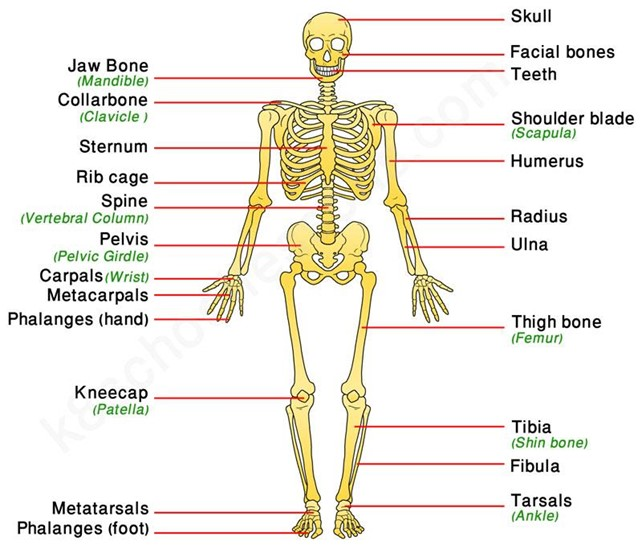
\includegraphics[width=\linewidth,keepaspectratio]{skeleton_divisions.jpg} 
		\end{center}	
    \end{column}
  \end{columns}
\end{frame}

%%%%%%%%%%%%%%%%%%%%%%%%%%%%%%%%%%%%%%%%%%%%%%%%%%%%%%%%%%%
\begin{frame}[fragile]\frametitle{Functions of skeleton system}

\begin{itemize}
\item Structural Framework
\item Support and protection
\item Blood formation
\item Storehouse of minerals
\end{itemize}
	  
\end{frame}


%%%%%%%%%%%%%%%%%%%%%%%%%%%%%%%%%%%%%%%%%%%%%%%%%%%%%%%%%%%
\begin{frame}[fragile]\frametitle{Vertebral Column}
\begin{columns}
    \begin{column}[T]{0.5\linewidth}
      \begin{itemize}
		\item Spine: Strong column of bone from head to lower back
		\item 33 vertebrae joined by cartilage and ligaments
		\item Spinal cord runs through central holes in vertebrae
		\item Vertebrae groups: Cervical (7), Thoracic (12), Lumbar (5)
		\item Sacral (5 fused into 1), Coccygeal (4 fused into 1)
		\item Curvatures: Cervical, Thoracic, Lumbar, Pelvic
		\item Improper posture can exaggerate spinal curves
		\item Kyphosis: Increased thoracic curve
		\item Lordosis: Exaggerated lumbar curve
		\item Scoliosis: Lateral curvature of the spine
		\item Asanas can help correct posture by balancing and strengthening muscles
	  \end{itemize}
    \end{column}
    \begin{column}[T]{0.5\linewidth}
		\begin{center}
		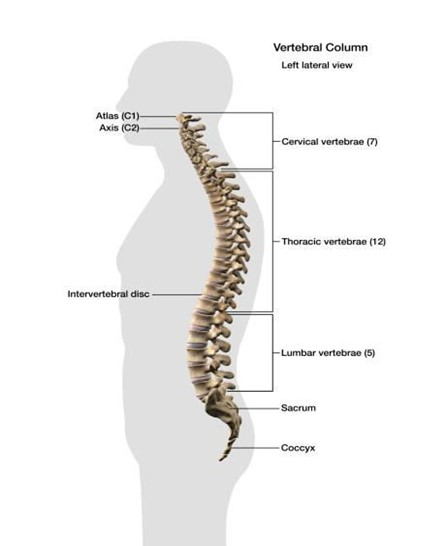
\includegraphics[width=\linewidth,keepaspectratio]{vertebral_column.jpg} 
		\end{center}	
    \end{column}
  \end{columns}
\end{frame}

%%%%%%%%%%%%%%%%%%%%%%%%%%%%%%%%%%%%%%%%%%%%%%%%%%%%%%%%%%%
\begin{frame}[fragile]\frametitle{Types of Spinal Movements}
\begin{columns}
    \begin{column}[T]{0.5\linewidth}
      \begin{itemize}
		\item Flexion: Forward bending; maximal in cervical region (e.g., Paschimotanasana, Padahastasana)
		\item Extension: Back bending (e.g., Bhujangasana, Dhanurasana)
		\item Rotation: Longitudinal twisting; greatest between atlas and axis (e.g., Ardha Matsyendrasana)
		\item Sideways Bending: Maximal in cervical and lumbar regions (e.g., Trikonasana)
		\item Circumduction: Swaying combining all movements (e.g., Chakki Chalavan)
		\item Elongation: Stretching upwards from base of spine (e.g., Tadasana, Urdhvahasta Dandasana)
	  \end{itemize}
    \end{column}
    \begin{column}[T]{0.5\linewidth}
		\begin{center}
		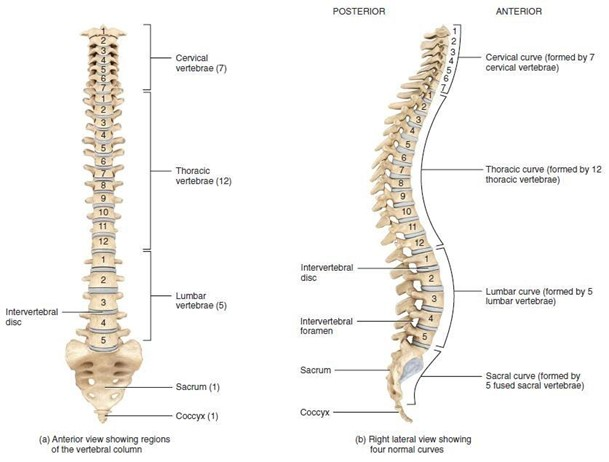
\includegraphics[width=\linewidth,keepaspectratio]{spinal_movements.jpg} 
		\end{center}	
    \end{column}
  \end{columns}
\end{frame}

%%%%%%%%%%%%%%%%%%%%%%%%%%%%%%%%%%%%%%%%%%%%%%%%%%%%%%%%%%%
\begin{frame}[fragile]\frametitle{Types of Joints}
\begin{columns}
    \begin{column}[T]{0.6\linewidth}
      \begin{itemize}
		\item Joints: Points of contact between two bones
		\item Fibrous Joints: Allow the least movement; e.g., sutures in skull
		\item Cartilaginous Joints: Bones connected by cartilage; e.g., ribs to sternum
		\item Synovial Joints: Highest mobility; coated with cartilage, contain synovial fluid
		\item Fibrous Joints: Immovable parts of the skeletal system
		\item Cartilaginous Joints: Strong but flexible, necessary movement (e.g., breathing)
		\item Synovial Joints: Sealed in fluid-filled joint capsule
		\item Six kinds of synovial joints for various movements
	  \end{itemize}
    \end{column}
    \begin{column}[T]{0.4\linewidth}
		\begin{center}
		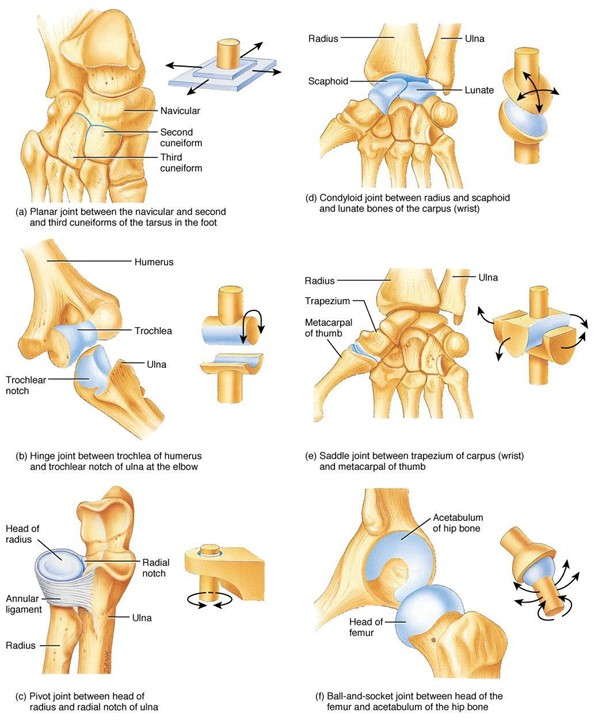
\includegraphics[width=\linewidth,keepaspectratio]{joints.jpg} 
		\end{center}	
    \end{column}
  \end{columns}
\end{frame}

%%%%%%%%%%%%%%%%%%%%%%%%%%%%%%%%%%%%%%%%%%%%%%%%%%%%%%%%%%%
\begin{frame}[fragile]\frametitle{Muscular System Overview}
\begin{columns}
    \begin{column}[T]{0.5\linewidth}
      \begin{itemize}
		\item Muscles are contractile tissues.
		\item They convert chemical energy into mechanical energy.
		\item Three types of muscles: voluntary, involuntary, cardiac.
		\item Voluntary muscles: consciously controlled.
		\item Involuntary muscles: controlled by autonomic nervous system.
		\item Cardiac muscle: auto rhythmic, contracts without stimulation.
		\item Voluntary muscles aid in walking, balancing, writing.
		\item Involuntary muscles help in digestion, blood flow.
		\item Cardiac muscle is specialized for heart function.
	  \end{itemize}
    \end{column}
    \begin{column}[T]{0.5\linewidth}
		\begin{center}
		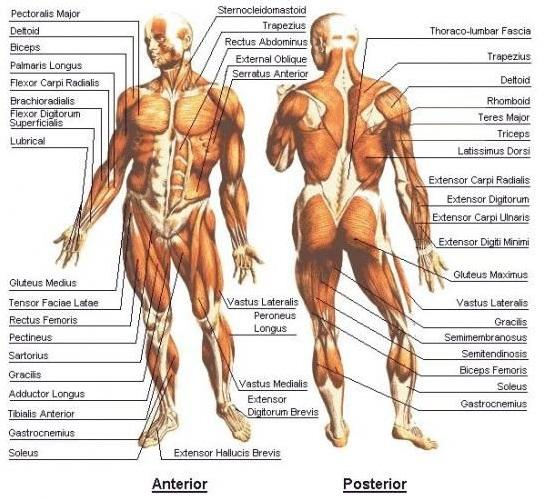
\includegraphics[width=\linewidth,keepaspectratio]{Muscle-chart-showing-the-muscular-system-labeled.jpg}
						
		{\tiny (Ref: https://www.biologyonline.com/dictionary/muscular-system)}			
		\end{center}	
    \end{column}
  \end{columns}
\end{frame}


%%%%%%%%%%%%%%%%%%%%%%%%%%%%%%%%%%%%%%%%%%%%%%%%%%%%%%%%%%%
\begin{frame}[fragile]\frametitle{Functions of Muscular System }

      \begin{itemize}
		\item Production of movement. Maintaining posture against gravity.
		\item Protection of internal organs
		\item Heat production
		\item Store for energy (protein and carbohydrates)
		\item Functioning of internal organs because of involuntary muscles.
	  \end{itemize}

\end{frame}

%%%%%%%%%%%%%%%%%%%%%%%%%%%%%%%%%%%%%%%%%%%%%%%%%%%%%%%%%%%
\begin{frame}[fragile]\frametitle{Muscle Contraction}
\begin{columns}
    \begin{column}[T]{0.5\linewidth}
      \begin{itemize}
		\item Muscles consist of fibres wrapped in a sheath.
		\item Muscle fibres contain actin (thin) and myosin (thick) filaments.
		\item Filaments overlap to create tension and shorten muscle fibres.
		\item Relaxed muscles: minimal overlap of filaments.
		\item Stimulated muscles: filaments slide and overlap, causing contraction.
		\item Maximal contraction: complete overlap of filaments.
		\item Muscle strength increases through more fibre engagement or efficiency.
		\item Isotonic Contraction: muscle changes shape while load remains constant.
		\item Isometric Contraction: muscle stays same size while load increases.
	  \end{itemize}
    \end{column}
    \begin{column}[T]{0.5\linewidth}
		\begin{center}
		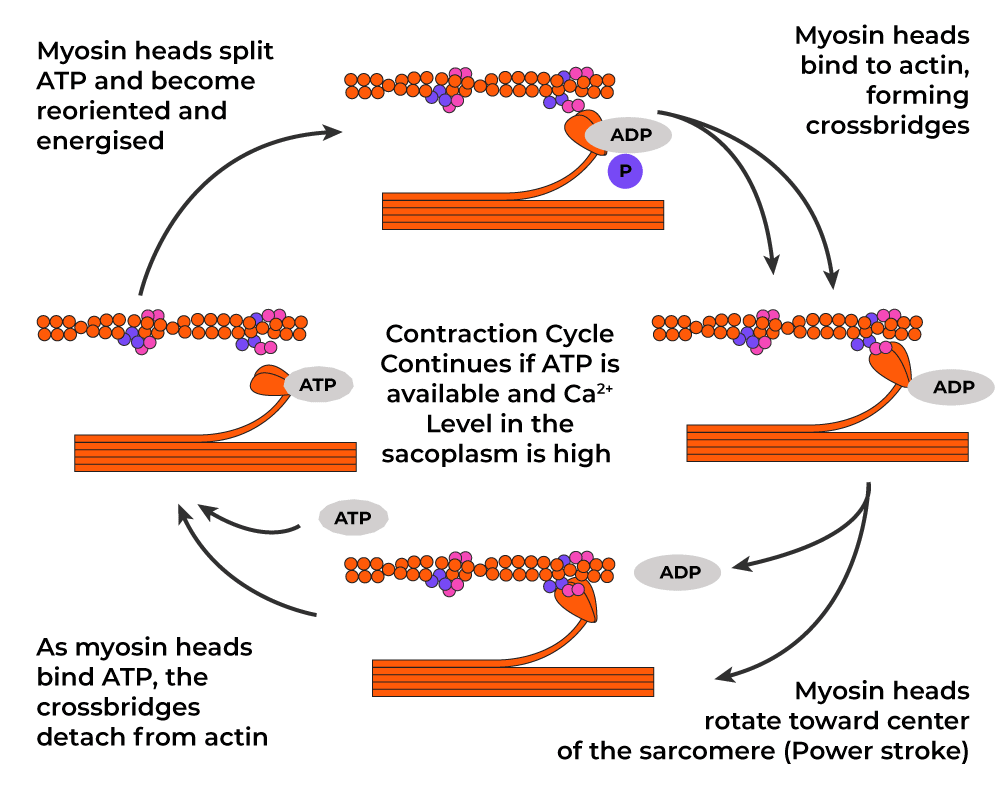
\includegraphics[width=\linewidth,keepaspectratio]{Mechnaism-of-muscle-contrtaction.png}
		
		
						
		{\tiny (Ref: https://www.geeksforgeeks.org/mechanism-of-muscle-contraction-class-11/)}		
		\end{center}	
    \end{column}
  \end{columns}
\end{frame}

%%%%%%%%%%%%%%%%%%%%%%%%%%%%%%%%%%%%%%%%%%%%%%%%%%%%%%%%%%%
\begin{frame}[fragile]\frametitle{Reflex Action \& Reciprocal Inhibition}
\begin{columns}
    \begin{column}[T]{0.5\linewidth}
      \begin{itemize}
		\item Motor units: smallest nerve fibre groups in muscles.
		\item Proprioceptors: sensors that send body position info to the brain.
		\item Proprioception aids in posture and coordination.
		\item Stretch reflex: strong contraction when muscle is suddenly lengthened.
		\item Example: back muscles contract when bending forward quickly.
		\item Slow movements support deep breathing.
		\item Reciprocal inhibition: opposing muscles relax when one contracts.
		\item Example: biceps contract, triceps relax.
		\item Ensures smooth and coordinated muscle movements.
	  \end{itemize}
    \end{column}
    \begin{column}[T]{0.5\linewidth}
		\begin{center}
		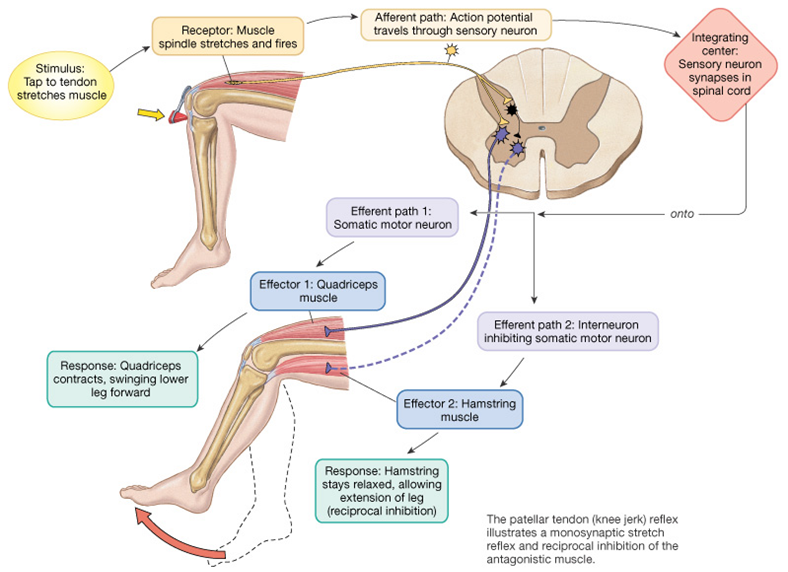
\includegraphics[width=\linewidth,keepaspectratio]{Reciprocal-Inhibition.png}
		
						
		{\tiny (Ref: https://www.corewalking.com/reciprocal-inhibition/)}
		\end{center}	
    \end{column}
  \end{columns}
\end{frame}

%%%%%%%%%%%%%%%%%%%%%%%%%%%%%%%%%%%%%%%%%%%%%%%%%%%%%%%%%%%
\begin{frame}[fragile]\frametitle{Types of Muscle Movements}
\begin{columns}
    \begin{column}[T]{0.5\linewidth}
      \begin{itemize}
		\item Flexion: Decreases joint angle, e.g., bending the elbow.
		\item Extension: Increases joint angle, e.g., straightening the elbow.
		\item Abduction: Moves bone away from midline, e.g., lifting arms.
		\item Adduction: Moves bone towards midline, e.g., bringing legs together.
		\item Elevation: Movement upward, e.g., shrugging shoulders.
		\item Depression: Movement downward, e.g., lowering shoulders.
		\item Pronation: Palms face down.
		\item Supination: Palms face up.
		\item Rotation: Movement around an axis, e.g., internal or external rotation.
		\item Sphincter opening: Reduces or increases size of an opening.
	  \end{itemize}
    \end{column}
    \begin{column}[T]{0.5\linewidth}
		\begin{center}
		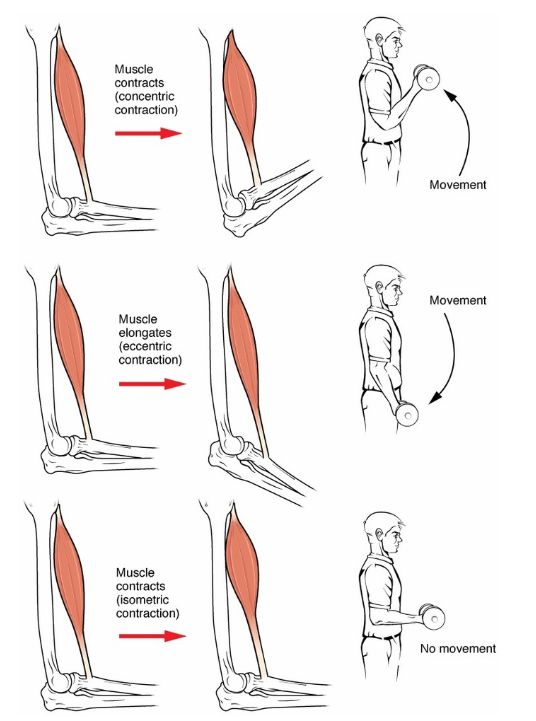
\includegraphics[width=\linewidth,keepaspectratio]{muscletypes}
				
		{\tiny (Ref: https://med.libretexts.org/Bookshelves/Anatomy\_and\_Physiology/}		
		\end{center}	
    \end{column}
  \end{columns}
\end{frame}

%%%%%%%%%%%%%%%%%%%%%%%%%%%%%%%%%%%%%%%%%%%%%%%%%%%%%%%%%%%
\begin{frame}[fragile]\frametitle{Muscle Breathing}
\begin{columns}
    \begin{column}[T]{0.5\linewidth}
      \begin{itemize}
		\item Muscles need energy for contraction.
		\item Energy comes from glucose metabolism using oxygen.
		\item Aerobic respiration: used in low-intensity, high-volume activities.
		\item Example: marathon running, dance.
		\item Anaerobic respiration: used when oxygen is insufficient or activities are very fast.
		\item Anaerobic respiration produces lactic acid as a byproduct.
		\item Example: weight training, sprints.
		\item Post-exertion: oxygen breaks down lactic acid into water and carbon dioxide.
		\item Oxygen debt: amount of oxygen required to break down lactic acid.
	  \end{itemize}
    \end{column}
    \begin{column}[T]{0.5\linewidth}
		\begin{center}
		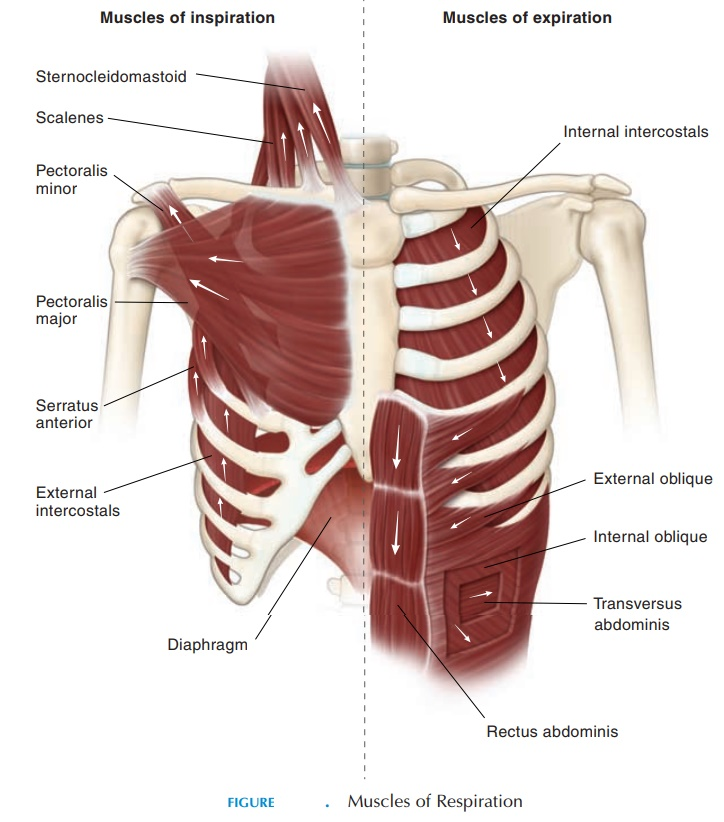
\includegraphics[width=\linewidth,keepaspectratio]{article-Respiration-Muscles-WC1.jpg}
				
		{\tiny (Ref: https://www.brainkart.com/article/Respiration-Muscles\_21121/)}
		\end{center}	
    \end{column}
  \end{columns}
\end{frame}

%%%%%%%%%%%%%%%%%%%%%%%%%%%%%%%%%%%%%%%%%%%%%%%%%%%%%%%%%%%
\begin{frame}[fragile]\frametitle{Cardiovascular System}
\begin{columns}
    \begin{column}[T]{0.5\linewidth}
      \begin{itemize}
		\item Cardiovascular system transports nutrients, gases, waste, hormones.
		\item Blood consists of:
			\begin{itemize}
				\item Plasma (54\% of blood mass)
				\item Red blood cells (45\%)
				\item White blood cells and platelets (1\%)
			\end{itemize}
		\item Red Blood Cells (RBCs): Transport oxygen and carbon dioxide.
		\item RBCs produced in bone marrow, lifespan ~120 days.
		\item Anaemia: Condition when RBC count falls below 30\%.
		\item White Blood Cells (WBCs): Provide immunity, lifespan 30 hours to 25 days.
		\item Platelets: Prevent bleeding by sticking to damaged vessels.
		\item Platelets' average lifespan is 4 days.
	  \end{itemize}
    \end{column}
    \begin{column}[T]{0.5\linewidth}
		\begin{center}
		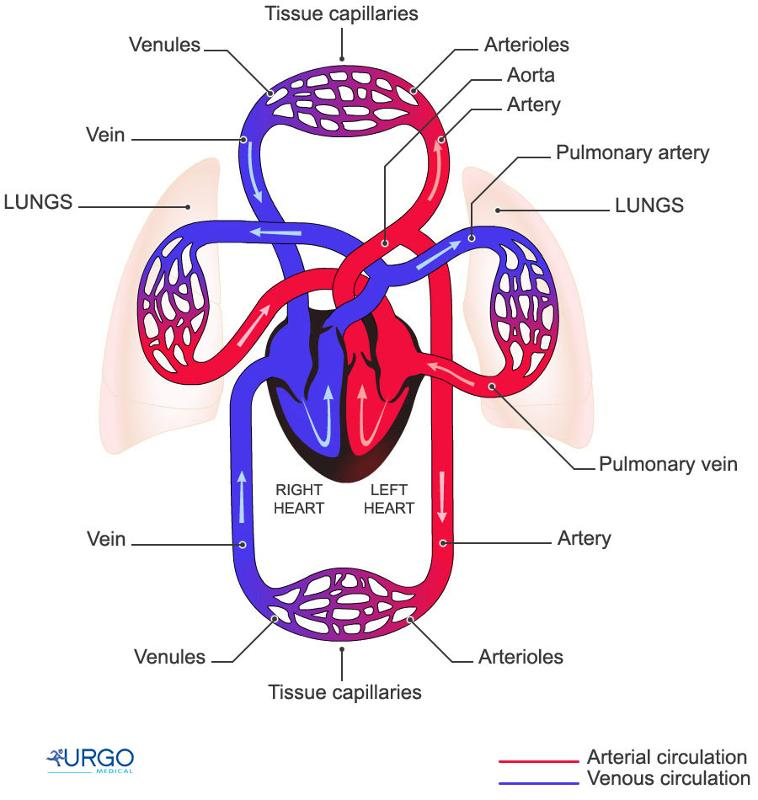
\includegraphics[width=\linewidth,keepaspectratio]{CardiovascularSystem.jpg}
		
				
		{\tiny (Ref: https://www.meresearch.org.uk/taking-heart-1/)}		
		\end{center}	
    \end{column}
  \end{columns}
\end{frame}

%%%%%%%%%%%%%%%%%%%%%%%%%%%%%%%%%%%%%%%%%%%%%%%%%%%%%%%%%%%
\begin{frame}[fragile]\frametitle{Blood Vessels \& Heart}
\begin{columns}
    \begin{column}[T]{0.5\linewidth}
      \begin{itemize}
		\item Blood vessels transport blood throughout the body.
		\item Arteries carry blood away from the heart.
		\item Arteries branch into arterioles, then into capillaries for nutrient exchange.
		\item Capillaries converge into venules, which merge into veins.
		\item Veins carry blood back to the heart.
		\item Systemic circulation: blood flow to and from the body.
		\item Pulmonary circulation: blood flow to and from the lungs.
		\item Heart: muscular organ that pumps blood.
		\item Heart has 4 chambers: right atrium, left atrium, right ventricle, left ventricle.
		\item Atria receive blood; ventricles pump it out.
		\item Valves prevent backflow: tricuspid (right), bicuspid/mitral (left).
	  \end{itemize}
    \end{column}
    \begin{column}[T]{0.5\linewidth}
		\begin{center}
		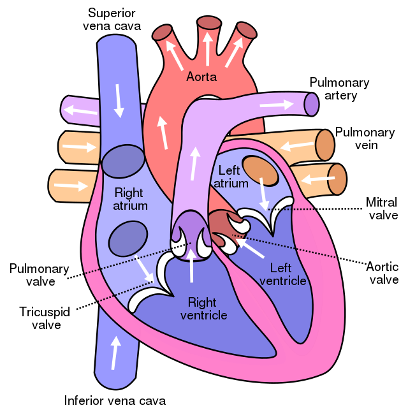
\includegraphics[width=\linewidth,keepaspectratio]{Heart-diagram.png}
				
		{\tiny (Ref: https://www.meresearch.org.uk/taking-heart-1/)}
		\end{center}	
    \end{column}
  \end{columns}
\end{frame}

%%%%%%%%%%%%%%%%%%%%%%%%%%%%%%%%%%%%%%%%%%%%%%%%%%%%%%%%%%%
\begin{frame}[fragile]\frametitle{Functions of Muscular System }

      \begin{itemize}
		\item Transport, blood circulation.
		\item Protection, immunity.
		\item Homeostasis.
	  \end{itemize}

\end{frame}

%%%%%%%%%%%%%%%%%%%%%%%%%%%%%%%%%%%%%%%%%%%%%%%%%%%%%%%%%%%
\begin{frame}[fragile]\frametitle{Respiratory System}
\begin{columns}
    \begin{column}[T]{0.5\linewidth}
      \begin{itemize}
		\item Respiration: Exchange of oxygen and carbon dioxide.
		\item At pulmonary level: Oxygen diffuses into capillaries, CO₂ into alveoli.
		\item At systemic level: Gas exchange occurs in capillaries near cells.
		\item Respiratory tract: Pathway for air to and from the lungs.
		\item Nose: Filters, warms, and moistens air; sense organ for smell.
		\item Pharynx: Passage from mouth and nose; connects to larynx.
		\item Larynx: Voice box; produces sound.
		\item Trachea: Windpipe; held open by cartilage rings.
		\item Bronchi, bronchioles, alveoli: Air passage branches ending in alveoli for gas exchange.
		\item Lungs: Triangular air sacs; two on the left (2 lobes), three on the right.
		\item Respiratory mucosa: Secretes mucus, traps irritants, and moves mucus to pharynx.
		\item Sinuses: Air-filled spaces around nasal cavity; prone to blockage and sinusitis.
	  \end{itemize}
    \end{column}
    \begin{column}[T]{0.5\linewidth}
		\begin{center}
		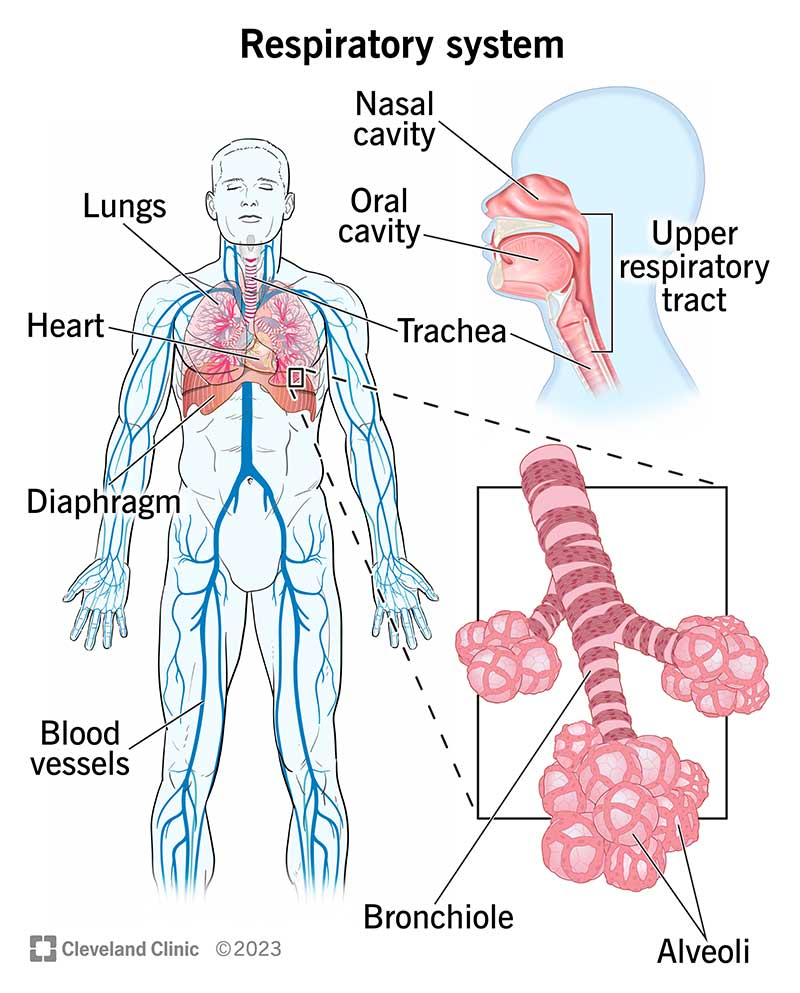
\includegraphics[width=\linewidth,keepaspectratio]{respiratory-system.jpg}
		\end{center}	
    \end{column}
  \end{columns}
\end{frame}
%%%%%%%%%%%%%%%%%%%%%%%%%%%%%%%%%%%%%%%%%%%%%%%%%%%%%%%%%%%
\begin{frame}[fragile]\frametitle{Functions of Muscular System }

      \begin{itemize}
		\item Exchange of gases
		\item Maintaining pH balance
		\item Speech production.
	  \end{itemize}

\end{frame}
	
%%%%%%%%%%%%%%%%%%%%%%%%%%%%%%%%%%%%%%%%%%%%%%%%%%%%%%%%%%%
\begin{frame}[fragile]\frametitle{Muscles of Respiration}
\begin{columns}
    \begin{column}[T]{0.5\linewidth}
      \begin{itemize}
		\item Diaphragm: Dome-shaped muscle below lungs; separates chest and abdominal cavities.
		\item Intercostal Muscles: Located between ribs; lift rib cage for inhalation, lower it for exhalation.
		\item Accessory Muscles: Neck muscles attached to collarbone; assist in clavicular breathing.
		\item Muscles of Expiration: Abdominal muscles; used for forceful exhalation.
	  \end{itemize}
    \end{column}
    \begin{column}[T]{0.5\linewidth}
		\begin{center}
		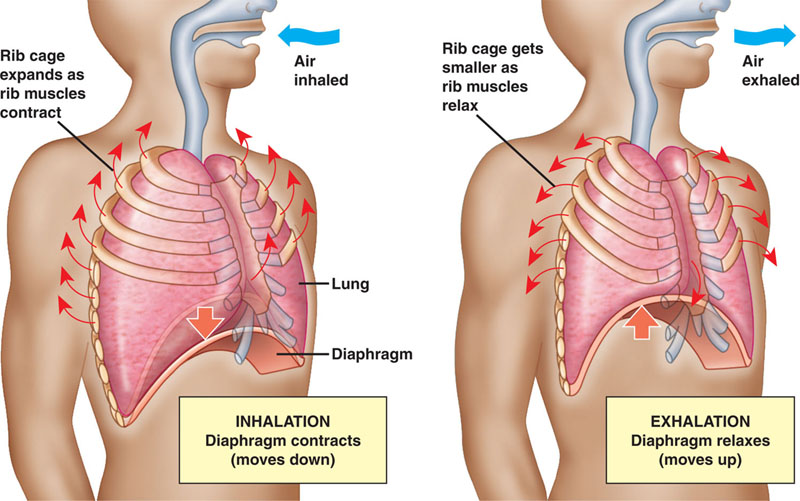
\includegraphics[width=\linewidth,keepaspectratio]{breathing.jpg}
		
		{\tiny (Ref: https://step1.medbullets.com/respiratory/117007/muscles-of-respiration)}
		\end{center}	
    \end{column}
  \end{columns}
\end{frame}

%%%%%%%%%%%%%%%%%%%%%%%%%%%%%%%%%%%%%%%%%%%%%%%%%%%%%%%%%%%
\begin{frame}[fragile]\frametitle{Digestive System}
\begin{columns}
    \begin{column}[T]{0.5\linewidth}
      \begin{itemize}
		\item Digestion: Breaking down complex molecules into simpler ones (glucose, fatty acids, amino acids).
		\item Alimentary Canal: 12 meters long muscular tube with mucosal lining.
		\item Food movement: By peristalsis (wave-like contractions).
		\item Mouth: Mechanical breakdown (chewing) and initial carbohydrate digestion by saliva.
		\item Oesophagus: Connects mouth to stomach; no digestion or absorption.
		\item Stomach: Mechanical breakdown and initial chemical digestion of proteins, fats, and milk. No absorption; secretes hydrochloric acid.
		\item Small Intestine: 6m long, divided into duodenum, jejunum, ileum; digestion and absorption of nutrients. Villi increase absorption surface area.
		\item Large Intestine: Absorbs water, forms feces; consists of ascending, transverse, descending colon, rectum, and anus.
	  \end{itemize}
    \end{column}
    \begin{column}[T]{0.5\linewidth}
		\begin{center}
		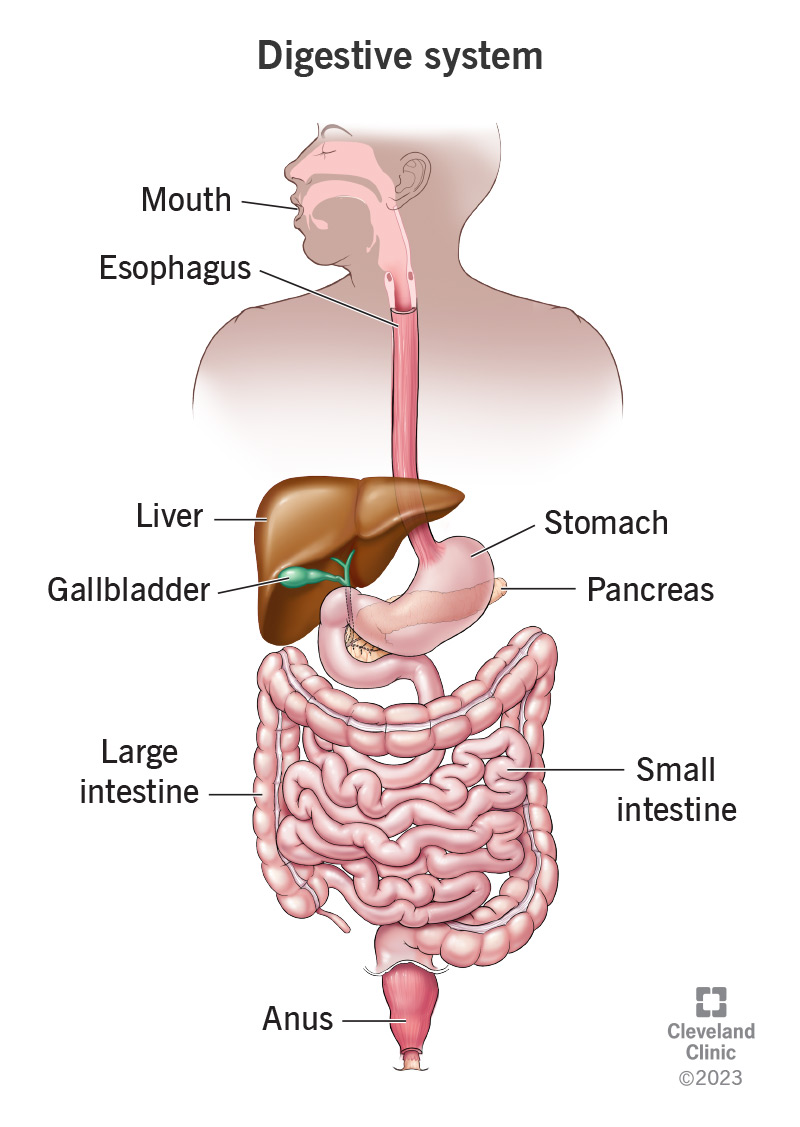
\includegraphics[width=\linewidth,keepaspectratio]{digestive-system.jpg}
		
		{\tiny (Ref: https://my.clevelandclinic.org/health/body/7041-digestive-system)}
		\end{center}	
    \end{column}
  \end{columns}
\end{frame}

%%%%%%%%%%%%%%%%%%%%%%%%%%%%%%%%%%%%%%%%%%%%%%%%%%%%%%%%%%%
\begin{frame}[fragile]\frametitle{Excretory System}
\begin{columns}
    \begin{column}[T]{0.5\linewidth}
      \begin{itemize}
		\item Kidneys: Bean-shaped organs that filter blood; contain ~1 million nephrons each.
		\item Ureters: Smooth muscle tubes that transport urine from kidneys to bladder via peristalsis.
		\item Urinary Bladder: Hollow organ that stores urine; holds 300-500 ml before the urge to urinate.
		\item Urethra: Tube connecting bladder to external orifice for urine expulsion.
	  \end{itemize}
    \end{column}
    \begin{column}[T]{0.5\linewidth}
		\begin{center}
		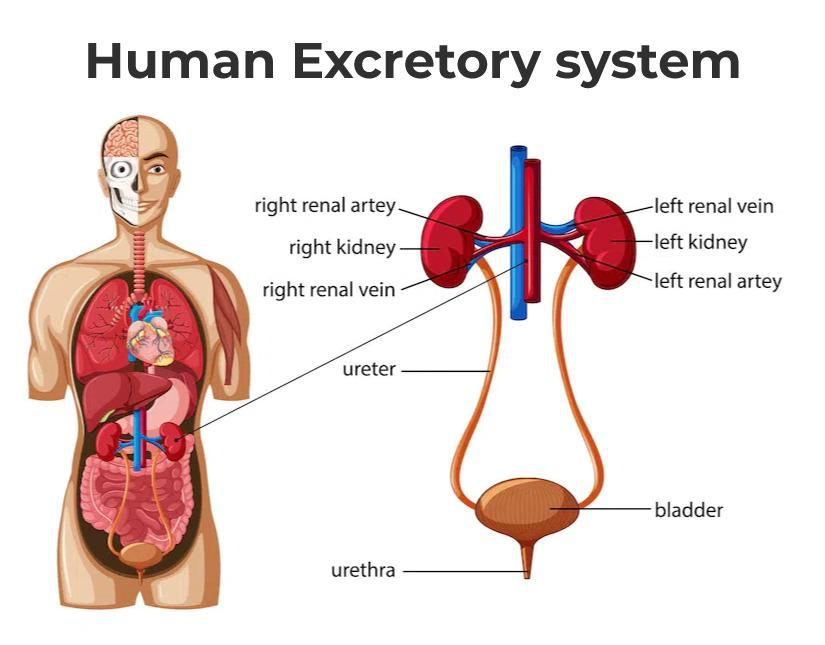
\includegraphics[width=\linewidth,keepaspectratio]{Human-Excretory-System.jpg}
		
		{\tiny (Ref: https://www.geeksforgeeks.org/diagram-of-excretory-system/)}
		\end{center}	
    \end{column}
  \end{columns}
\end{frame}
%%%%%%%%%%%%%%%%%%%%%%%%%%%%%%%%%%%%%%%%%%%%%%%%%%%%%%%%%%%
\begin{frame}[fragile]\frametitle{Functions of Muscular System }

      \begin{itemize}
		\item Eliminate waste from the body.
		\item Regulate blood volume and blood pressure.
		\item Control levels of electrolytes and metabolites
		\item Regulate blood pH.

	  \end{itemize}

\end{frame}

%%%%%%%%%%%%%%%%%%%%%%%%%%%%%%%%%%%%%%%%%%%%%%%%%%%%%%%%%%%
\begin{frame}[fragile]\frametitle{Endocrine System}
\begin{columns}
    \begin{column}[T]{0.5\linewidth}
      \begin{itemize}
		\item Endocrine System: Regulates body activities through hormones.
		\item Hormones: Chemical regulators secreted into the blood.
		\item Secreted directly into blood; act on specific target organs.
		\item Produced in small quantities; not stored in the body.
		\item Types: Water-soluble proteins and amines, lipid-soluble steroids.
		\item Imbalance: Excess or deficiency can lead to serious health issues.
	  \end{itemize}
    \end{column}
    \begin{column}[T]{0.5\linewidth}
		\begin{center}
		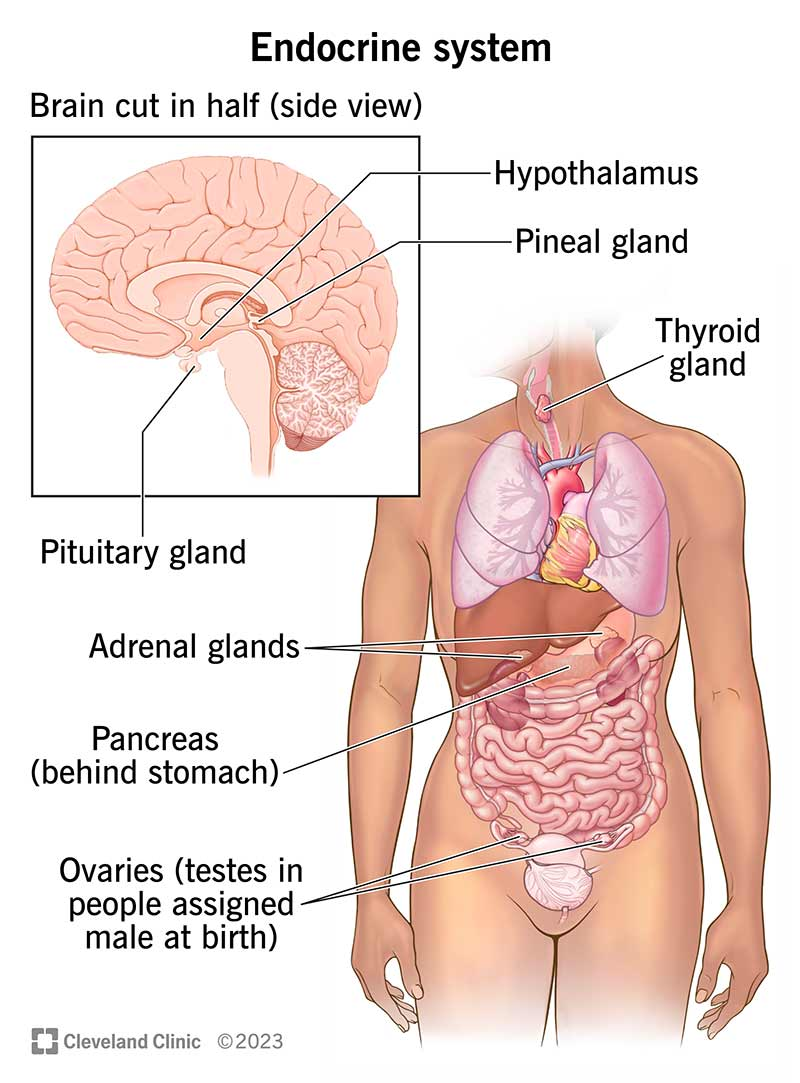
\includegraphics[width=\linewidth,keepaspectratio]{endocrine-system.jpg}
		\end{center}	
    \end{column}
  \end{columns}
\end{frame}

%%%%%%%%%%%%%%%%%%%%%%%%%%%%%%%%%%%%%%%%%%%%%%%%%%%%%%%%%%%
\begin{frame}[fragile]\frametitle{Endocrine Glands: Hypothalamus and Pituitary}
\begin{columns}
    \begin{column}[T]{0.5\linewidth}
      \begin{itemize}
		\item **Hypothalamus:** Directs pituitary gland.
		  \begin{itemize}
		    \item Releasing Hormone (RH): Stimulates pituitary hormone release.
		    \item Inhibiting Hormone (IH): Stops pituitary hormone release.
		  \end{itemize}
		\item **Pituitary Gland:** Master gland; regulates other endocrine glands.
		  \begin{itemize}
		    \item Growth Hormone (GH): Promotes growth.
		    \item Follicle Stimulating Hormone (FSH): Stimulates egg and sperm formation.
		    \item Luteinizing Hormone (LH): Stimulates corpus luteum and hormone production.
		    \item Prolactin: Milk secretion.
		    \item Thyroid Stimulating Hormone (TSH): Stimulates thyroid.
		    \item Adrenocorticotropic Hormone (ACTH): Stimulates adrenal glands.
		    \item Antidiuretic Hormone (ADH): Increases water reabsorption.
		    \item Oxytocin: Uterine contractions.
		  \end{itemize}
	  \end{itemize}
    \end{column}
    \begin{column}[T]{0.5\linewidth}
		\begin{center}
		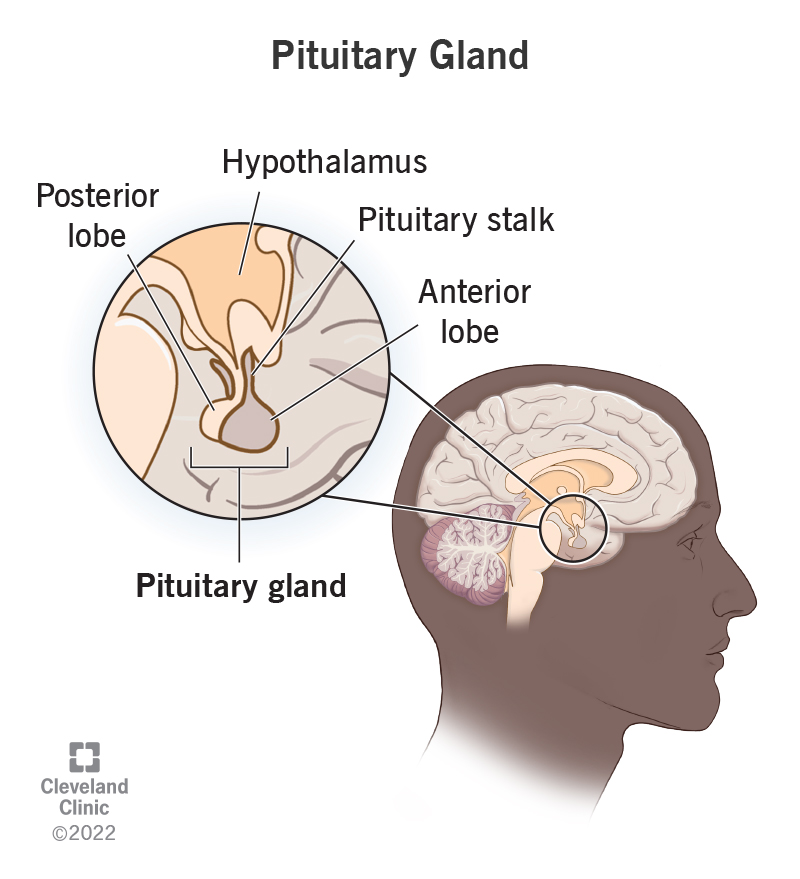
\includegraphics[width=\linewidth,keepaspectratio]{pituitary-gland.jpg}
		
		{\tiny (Ref: https://my.clevelandclinic.org/health/body/21459-pituitary-gland)}
		\end{center}	
    \end{column}
  \end{columns}
\end{frame}



%%%%%%%%%%%%%%%%%%%%%%%%%%%%%%%%%%%%%%%%%%%%%%%%%%%%%%%%%%%
\begin{frame}[fragile]\frametitle{Endocrine Glands: Pineal, Thyroid, and Parathyroid}
\begin{columns}
    \begin{column}[T]{0.5\linewidth}
      \begin{itemize}
		\item **Pineal Gland:** Produces melatonin; regulates sleep patterns.
		\item **Thyroid:** Produces thyroxin and calcitonin; regulates metabolism and calcium.
		\item **Parathyroid Glands:** Regulates calcium metabolism.
	  \end{itemize}
    \end{column}
    \begin{column}[T]{0.5\linewidth}
		\begin{center}
		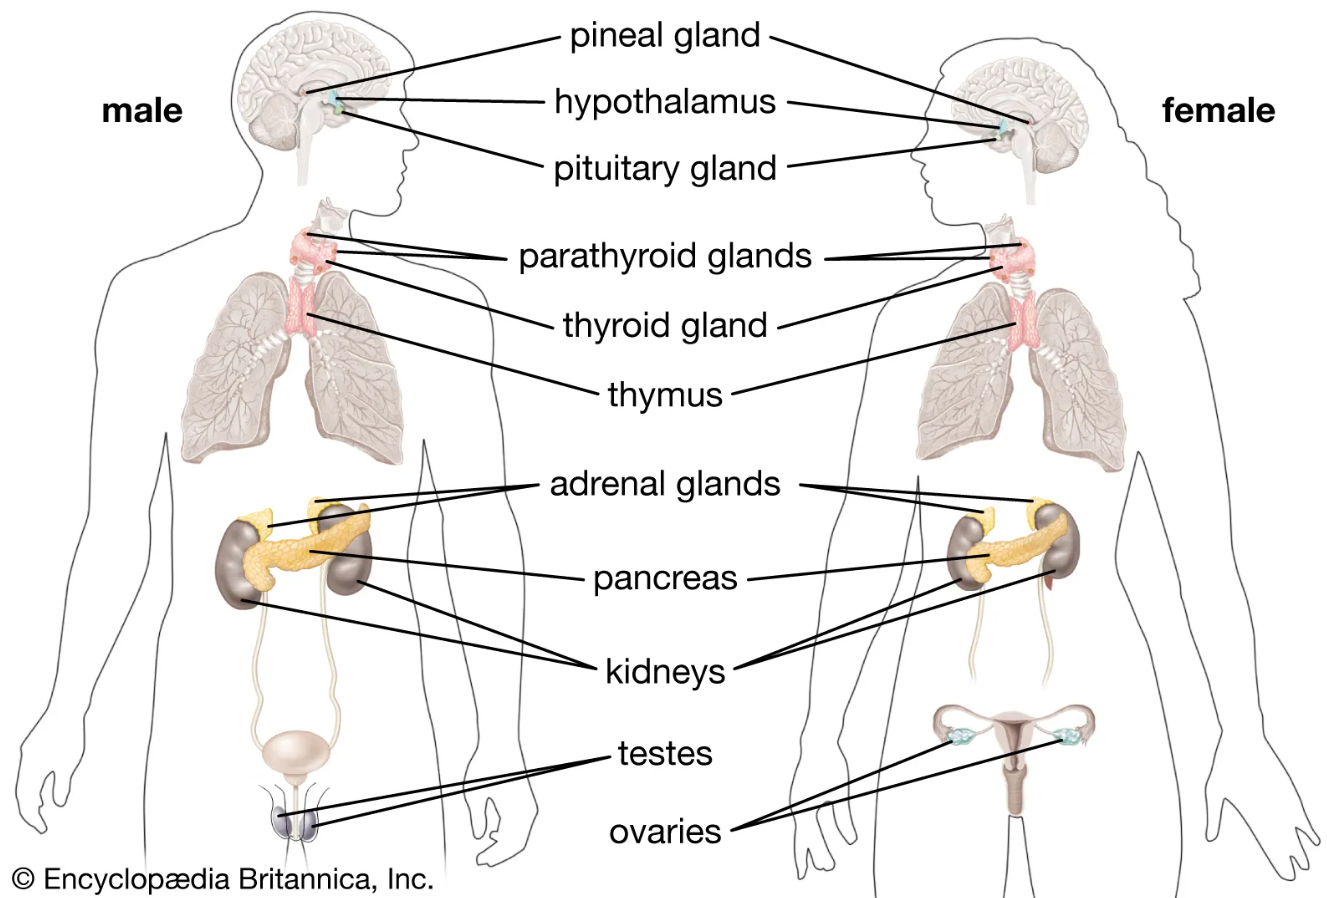
\includegraphics[width=\linewidth,keepaspectratio]{endocrine}
		\end{center}	
    \end{column}
  \end{columns}
\end{frame}

%%%%%%%%%%%%%%%%%%%%%%%%%%%%%%%%%%%%%%%%%%%%%%%%%%%%%%%%%%%
\begin{frame}[fragile]\frametitle{Overview of Reproductive System}
\begin{columns}
    \begin{column}[T]{0.5\linewidth}
      \begin{itemize}
		\item Essential for species survival.
		\item Humans procreate via sexual reproduction.
		\item Gametes: sperm (male) and egg (female).
		\item Fertilization forms a zygote.
		\item Zygote develops into an embryo, then a fetus.
	  \end{itemize}
    \end{column}
    \begin{column}[T]{0.5\linewidth}
		\begin{center}
		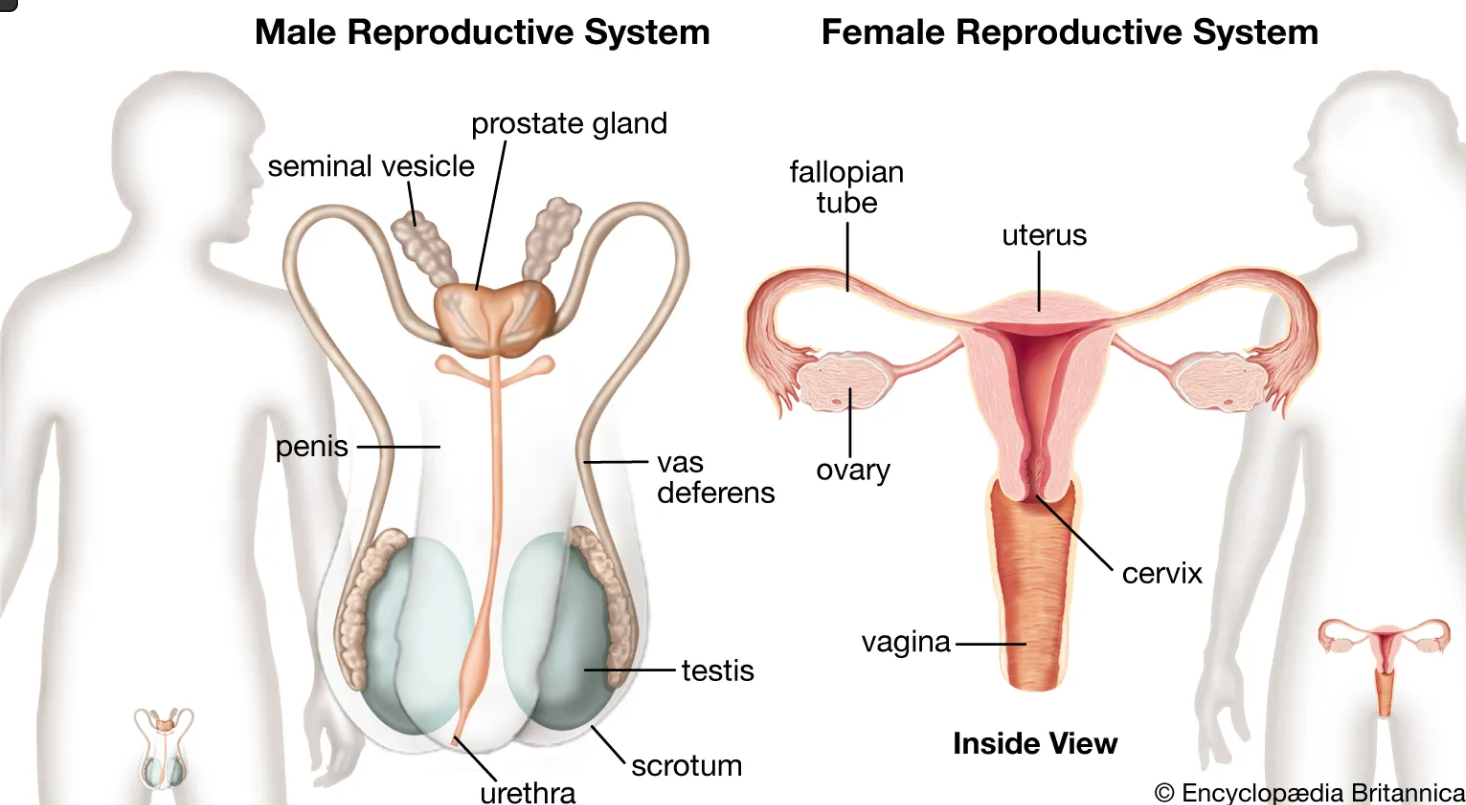
\includegraphics[width=\linewidth,keepaspectratio]{reprosys}

		
		{\tiny (Ref: https://www.britannica.com/science/human-reproductive-system)}		
		\end{center}	
    \end{column}
  \end{columns}
\end{frame}

%%%%%%%%%%%%%%%%%%%%%%%%%%%%%%%%%%%%%%%%%%%%%%%%%%%%%%%%%%%
\begin{frame}[fragile]\frametitle{Male Reproductive System}
\begin{columns}
    \begin{column}[T]{0.5\linewidth}
      \begin{itemize}
		\item Testes: Oval-shaped, produce sperm.
		\item Scrotum: Sac that holds testes.
		\item Seminal Vesicles: Produce seminal fluid.
		\item Prostate Gland: Adds fluids to semen.
		\item Penis: Passes urine and semen.
	  \end{itemize}
    \end{column}
    \begin{column}[T]{0.5\linewidth}
		\begin{center}
		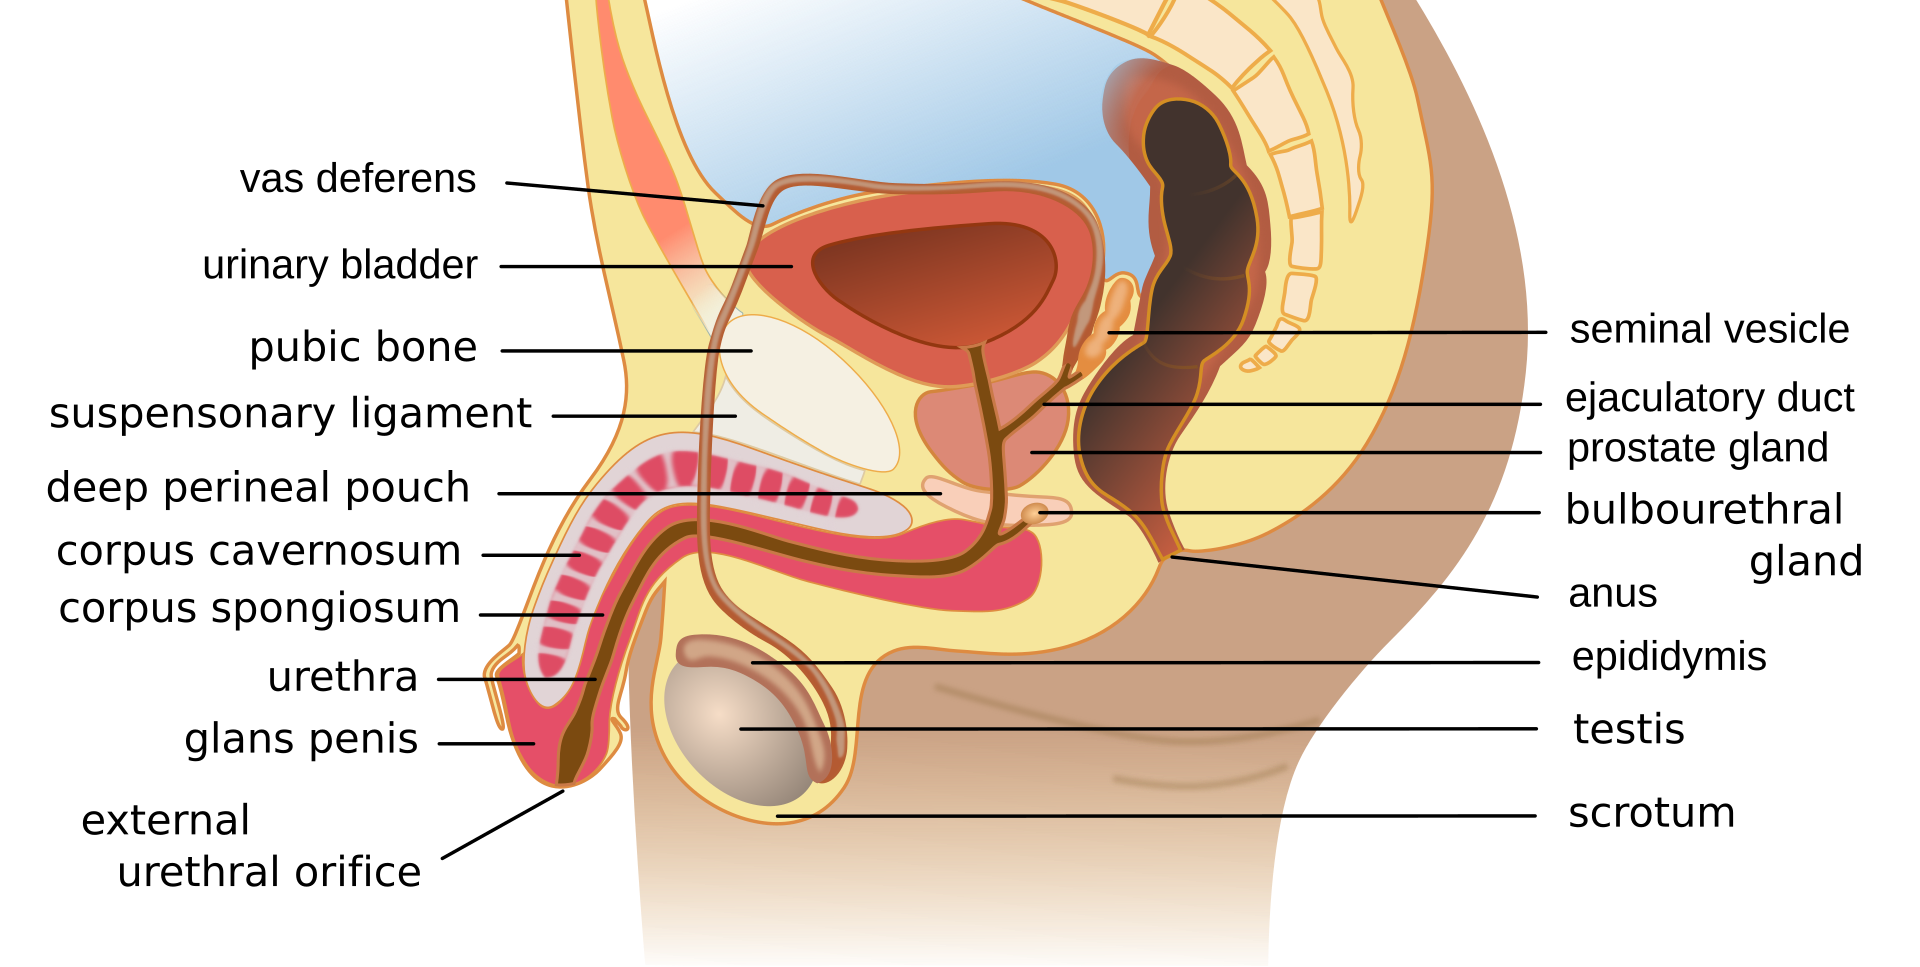
\includegraphics[width=\linewidth,keepaspectratio]{Human_male_reproductive_system_en.svg.png}
		
		{\tiny (Ref: https://simple.wikipedia.org/wiki/Male\_reproductive\_system)}
		\end{center}	
    \end{column}
  \end{columns}
\end{frame}

%%%%%%%%%%%%%%%%%%%%%%%%%%%%%%%%%%%%%%%%%%%%%%%%%%%%%%%%%%%
\begin{frame}[fragile]\frametitle{Female Reproductive System}
\begin{columns}
    \begin{column}[T]{0.5\linewidth}
      \begin{itemize}
		\item Key organs: Ovaries, oviducts, uterus, vagina.
		\item Functions: Egg production, fertilization, embryo development.
		\item Ovaries: Produce and mature eggs.
		\item Oviducts: Site of fertilization.
		\item Uterus: Houses and nurtures the embryo.
	  \end{itemize}
    \end{column}
    \begin{column}[T]{0.5\linewidth}
		\begin{center}
		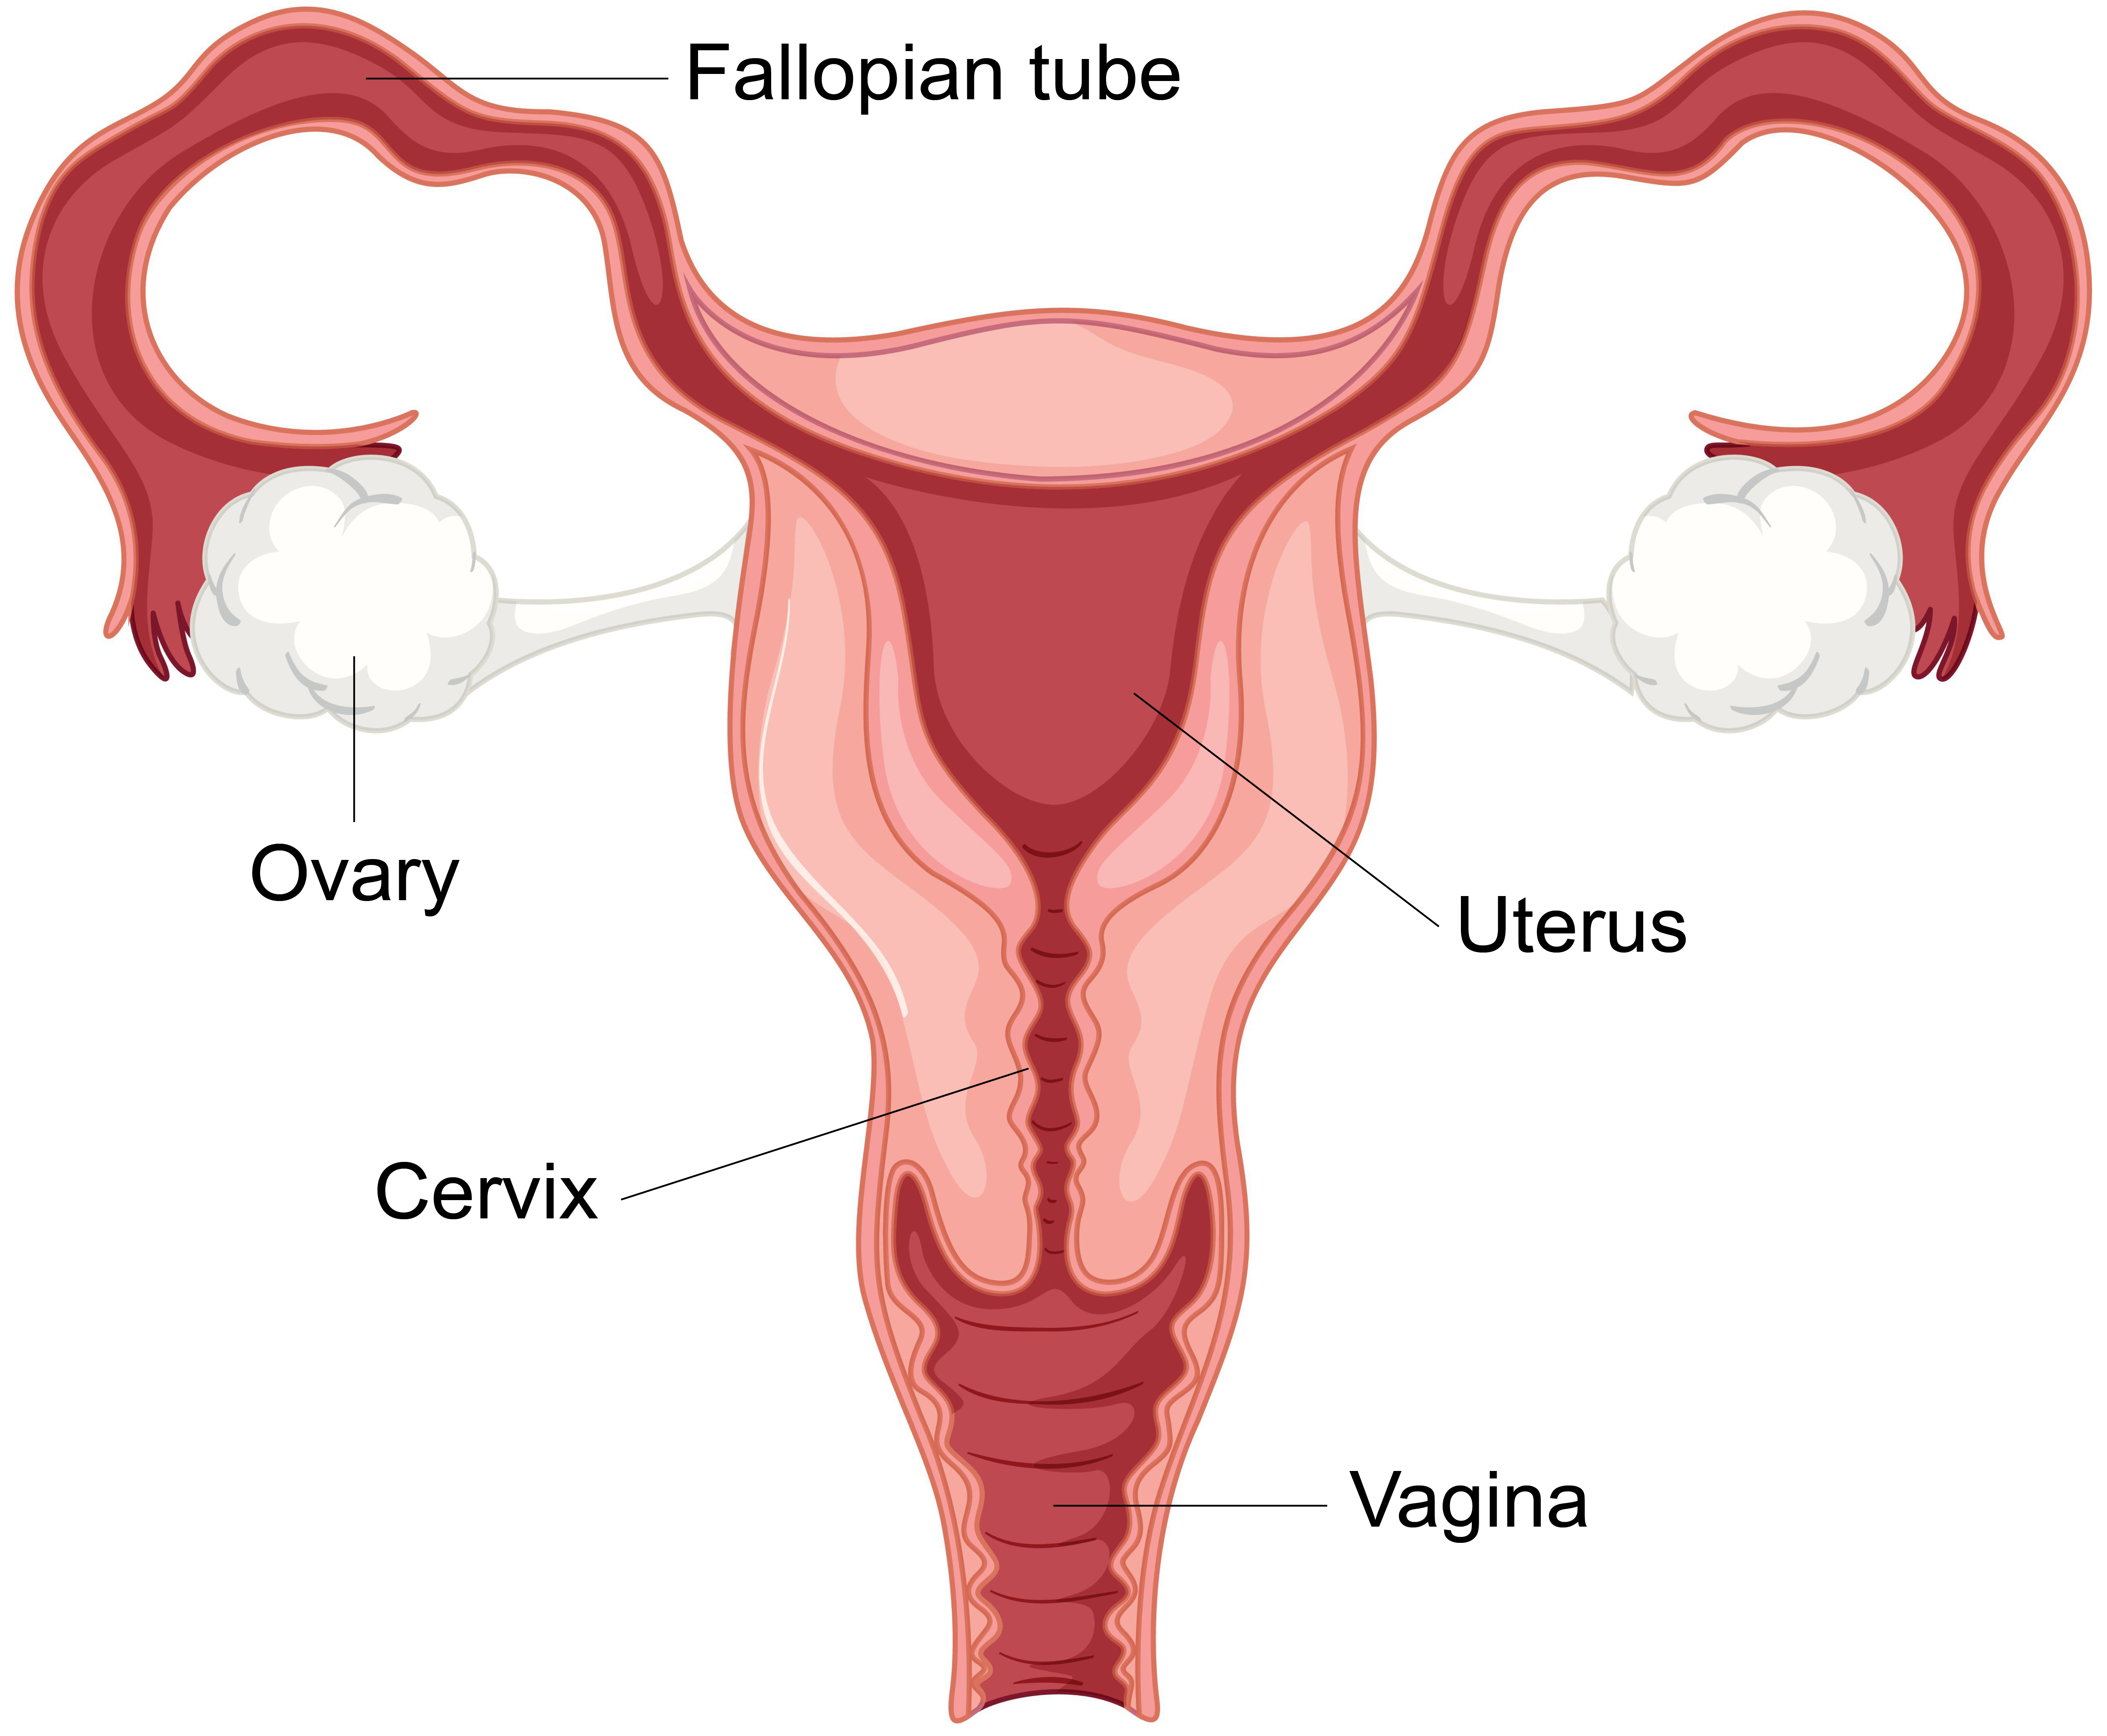
\includegraphics[width=\linewidth,keepaspectratio]{female-reproductive-system.jpg}
		
		{\tiny (Ref: https://www.healthdirect.gov.au/female-reproductive-system)}		
		\end{center}	
    \end{column}
  \end{columns}
\end{frame}

%%%%%%%%%%%%%%%%%%%%%%%%%%%%%%%%%%%%%%%%%%%%%%%%%%%%%%%%%%%
\begin{frame}[fragile]\frametitle{Overview of Nervous System}
\begin{columns}
    \begin{column}[T]{0.5\linewidth}
      \begin{itemize}
		\item Coordinates and controls body actions.
		\item Neuron: basic functional unit.
		\item Consists of CNS and PNS.
		\item CNS: Brain and spinal cord.
		\item PNS: Nerves connecting CNS to body.
	  \end{itemize}
    \end{column}
    \begin{column}[T]{0.5\linewidth}
		\begin{center}
		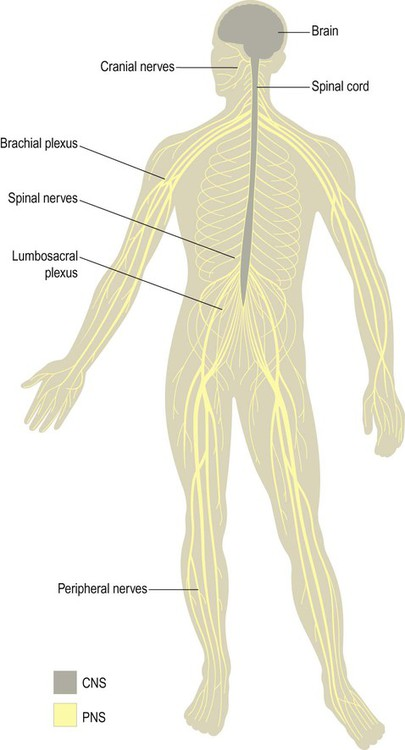
\includegraphics[width=\linewidth,keepaspectratio]{overview_nervious_system}
		
		{\tiny (Ref: https://neupsykey.com/overview-of-the-nervous-system/)}
		
		\end{center}	
    \end{column}
  \end{columns}
\end{frame}

%%%%%%%%%%%%%%%%%%%%%%%%%%%%%%%%%%%%%%%%%%%%%%%%%%%%%%%%%%%
\begin{frame}[fragile]\frametitle{Central Nervous System: Brain}
\begin{columns}
    \begin{column}[T]{0.5\linewidth}
      \begin{itemize}
		\item Brain: Protected by skull and meninges.
		\item Cerebrum: Largest part, divided into lobes.
		\item Cerebellum: Coordinates movements and balance.
		\item Medulla Oblongata: Controls vital functions.
		\item Diencephalon: Includes hypothalamus and thalamus.
	  \end{itemize}
    \end{column}
    \begin{column}[T]{0.5\linewidth}
		\begin{center}
		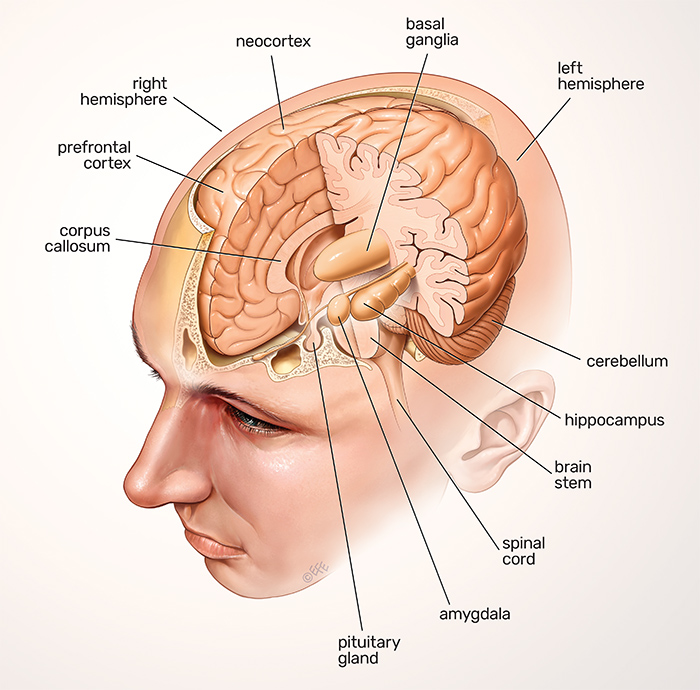
\includegraphics[width=\linewidth,keepaspectratio]{Basic-brain-anatomy.jpg}
		
		{\tiny (Ref: https://qbi.uq.edu.au/brain/brain-anatomy/central-nervous-system-brain-and-spinal-cord)}
		
		\end{center}	
    \end{column}
  \end{columns}
\end{frame}

%%%%%%%%%%%%%%%%%%%%%%%%%%%%%%%%%%%%%%%%%%%%%%%%%%%%%%%%%%%
\begin{frame}[fragile]\frametitle{Central Nervous System: Spinal Cord}
\begin{columns}
    \begin{column}[T]{0.5\linewidth}
      \begin{itemize}
		\item Extends from medulla oblongata to lumbar vertebra.
		\item Covered by meninges.
		\item Facilitates reflex actions.
		\item Conduction of sensory and motor impulses.
		\item Key role in communication between brain and body.
	  \end{itemize}
    \end{column}
    \begin{column}[T]{0.5\linewidth}
		\begin{center}
		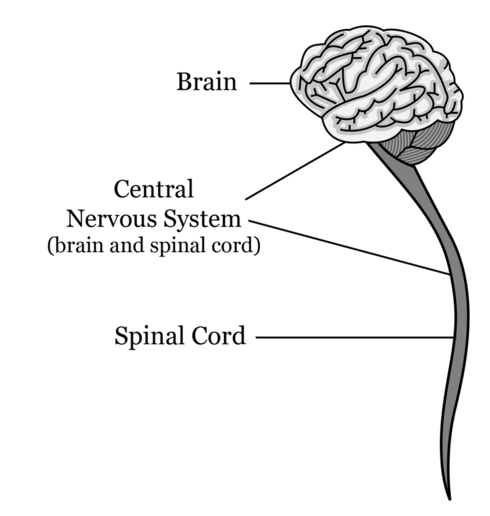
\includegraphics[width=\linewidth,keepaspectratio]{Spinal_chord}
		
		{\tiny (Ref: https://www.ck12.org/biology/central-nervous-system/lesson/central-nervous-system-ms-ls/)}
		\end{center}	
    \end{column}
  \end{columns}
\end{frame}

%%%%%%%%%%%%%%%%%%%%%%%%%%%%%%%%%%%%%%%%%%%%%%%%%%%%%%%%%%%
\begin{frame}[fragile]\frametitle{Peripheral Nervous System: Overview}
\begin{columns}
    \begin{column}[T]{0.5\linewidth}
      \begin{itemize}
		\item Includes all nerves outside CNS.
		\item Connects CNS to limbs and organs.
		\item Divided into Somatic and Autonomic systems.
		\item Somatic: Controls voluntary movements.
		\item Autonomic: Regulates involuntary functions.
	  \end{itemize}
    \end{column}
    \begin{column}[T]{0.5\linewidth}
		\begin{center}
		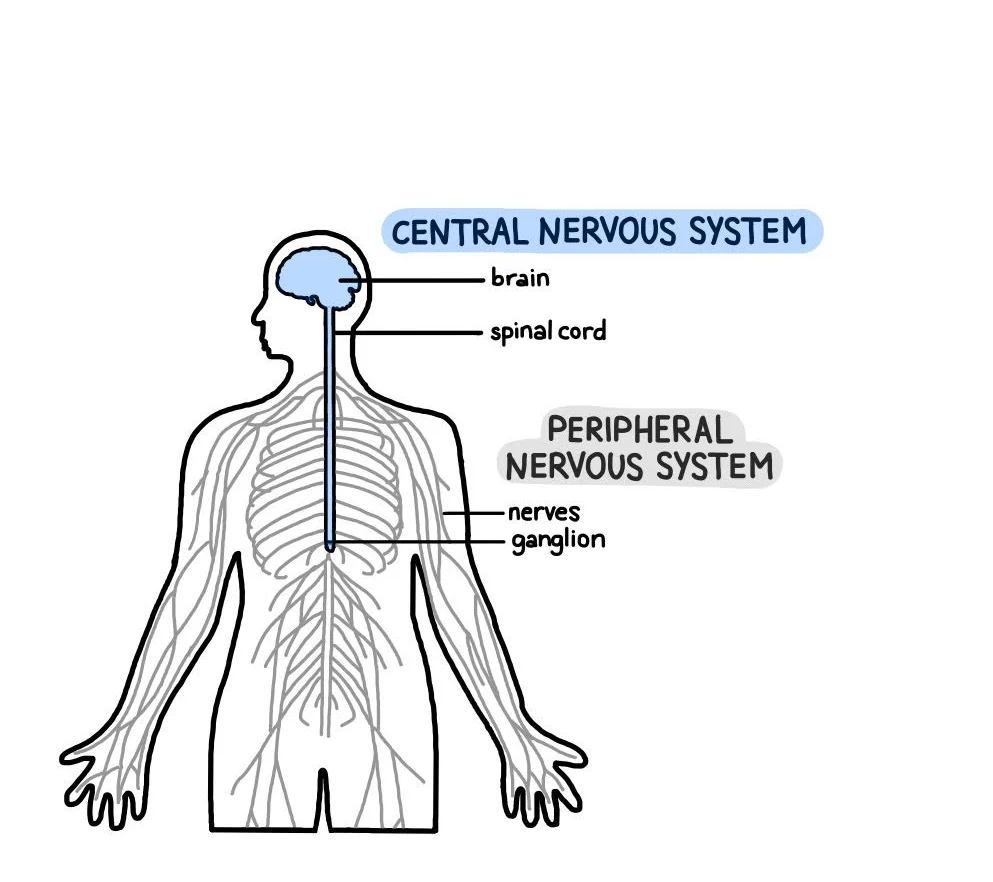
\includegraphics[width=\linewidth,keepaspectratio]{Peripheral_Nervous_System}
		
		{\tiny (Ref: https://www.simplypsychology.org/peripheral-nervous-system.html)}		
		\end{center}	
    \end{column}
  \end{columns}
\end{frame}

%%%%%%%%%%%%%%%%%%%%%%%%%%%%%%%%%%%%%%%%%%%%%%%%%%%%%%%%%%%
\begin{frame}[fragile]\frametitle{Somatic Nervous System (SNS)}
\begin{columns}
    \begin{column}[T]{0.5\linewidth}
      \begin{itemize}
		\item Sensory nerves: Carry impulses to CNS.
		\item Motor nerves: Carry impulses from CNS.
		\item 12 pairs of cranial nerves.
		\item 31 pairs of spinal nerves.
		\item Controls voluntary movements.
	  \end{itemize}
    \end{column}
    \begin{column}[T]{0.5\linewidth}
		\begin{center}
		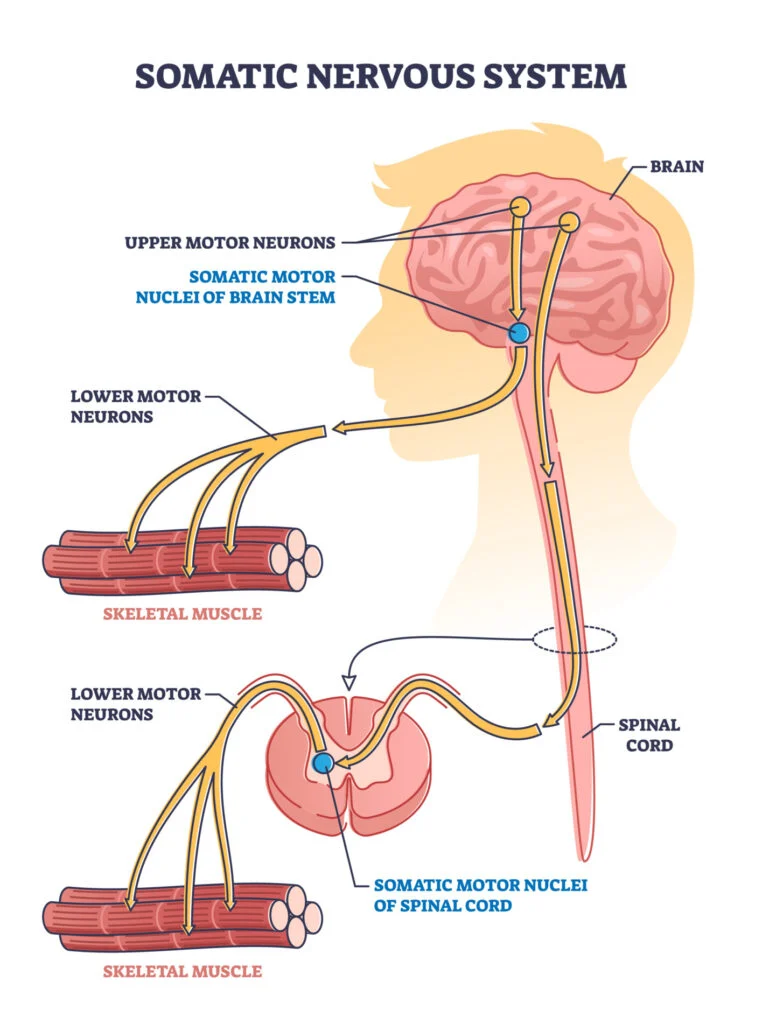
\includegraphics[width=\linewidth,keepaspectratio]{Somatic_nervous_system}
		
		{\tiny (Ref: https://www.simplypsychology.org/somatic-nervous-system.html)}
		\end{center}	
    \end{column}
  \end{columns}
\end{frame}

%%%%%%%%%%%%%%%%%%%%%%%%%%%%%%%%%%%%%%%%%%%%%%%%%%%%%%%%%%%
\begin{frame}[fragile]\frametitle{Autonomic Nervous System (ANS)}
\begin{columns}
    \begin{column}[T]{0.5\linewidth}
      \begin{itemize}
		\item Regulates involuntary actions.
		\item Sympathetic: 'Fight or flight' response.
		\item Parasympathetic: 'Rest and digest' response.
		\item Controls internal organs.
		\item Includes sympathetic and parasympathetic chains.
	  \end{itemize}
    \end{column}
    \begin{column}[T]{0.5\linewidth}
		\begin{center}
		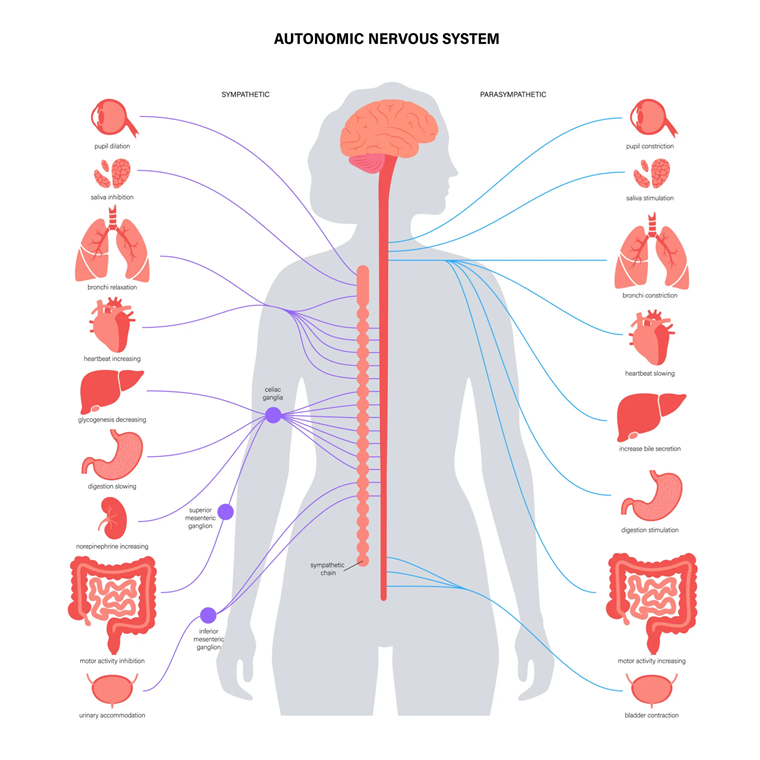
\includegraphics[width=\linewidth,keepaspectratio]{Autonomic_Nervous_System}
		
		{\tiny (Ref: https://www.simplypsychology.org/autonomic-nervous-system.html)}
		\end{center}	
    \end{column}
  \end{columns}
\end{frame}
